% !TEX program = xelatex
% Mapa da bancada: imprimir um para colar no switch e um por grupo.
\documentclass[11pt]{article}
\usepackage[brazil]{babel}
\usepackage[sfdefault,lf]{FiraSans}
\usepackage{FiraMono}
\usepackage[a4paper,landscape,margin=1.2cm]{geometry}
\usepackage[table]{xcolor}
\usepackage{array,tabularx,booktabs,graphicx}
\definecolor{Navy}{HTML}{111827}
\definecolor{Ciano}{HTML}{0B7F7D}
\definecolor{Ambar}{HTML}{B7791F}
\definecolor{Roxo}{HTML}{6B46C1}
\definecolor{Cinza}{HTML}{5B6677}
\definecolor{Vermelho}{HTML}{C53030}
\definecolor{RuleGray}{HTML}{C9D1DB}
\pagestyle{empty}
\setlength{\parindent}{0pt}
\arrayrulecolor{RuleGray}
\renewcommand{\arraystretch}{1.3}
\newcommand{\cab}[1]{\textcolor{white}{\bfseries #1}}
\newcommand{\cel}[1]{\cellcolor{#1}\color{white}\bfseries}

\begin{document}

{\color{Navy}\bfseries\LARGE Rede da planta: mapa da bancada}\hfill{\color{Cinza}Monitoria de Redes, UFPE, Aula 3}

\vspace{0.3cm}
\begin{minipage}[t]{0.47\textwidth}
\vspace{0pt}
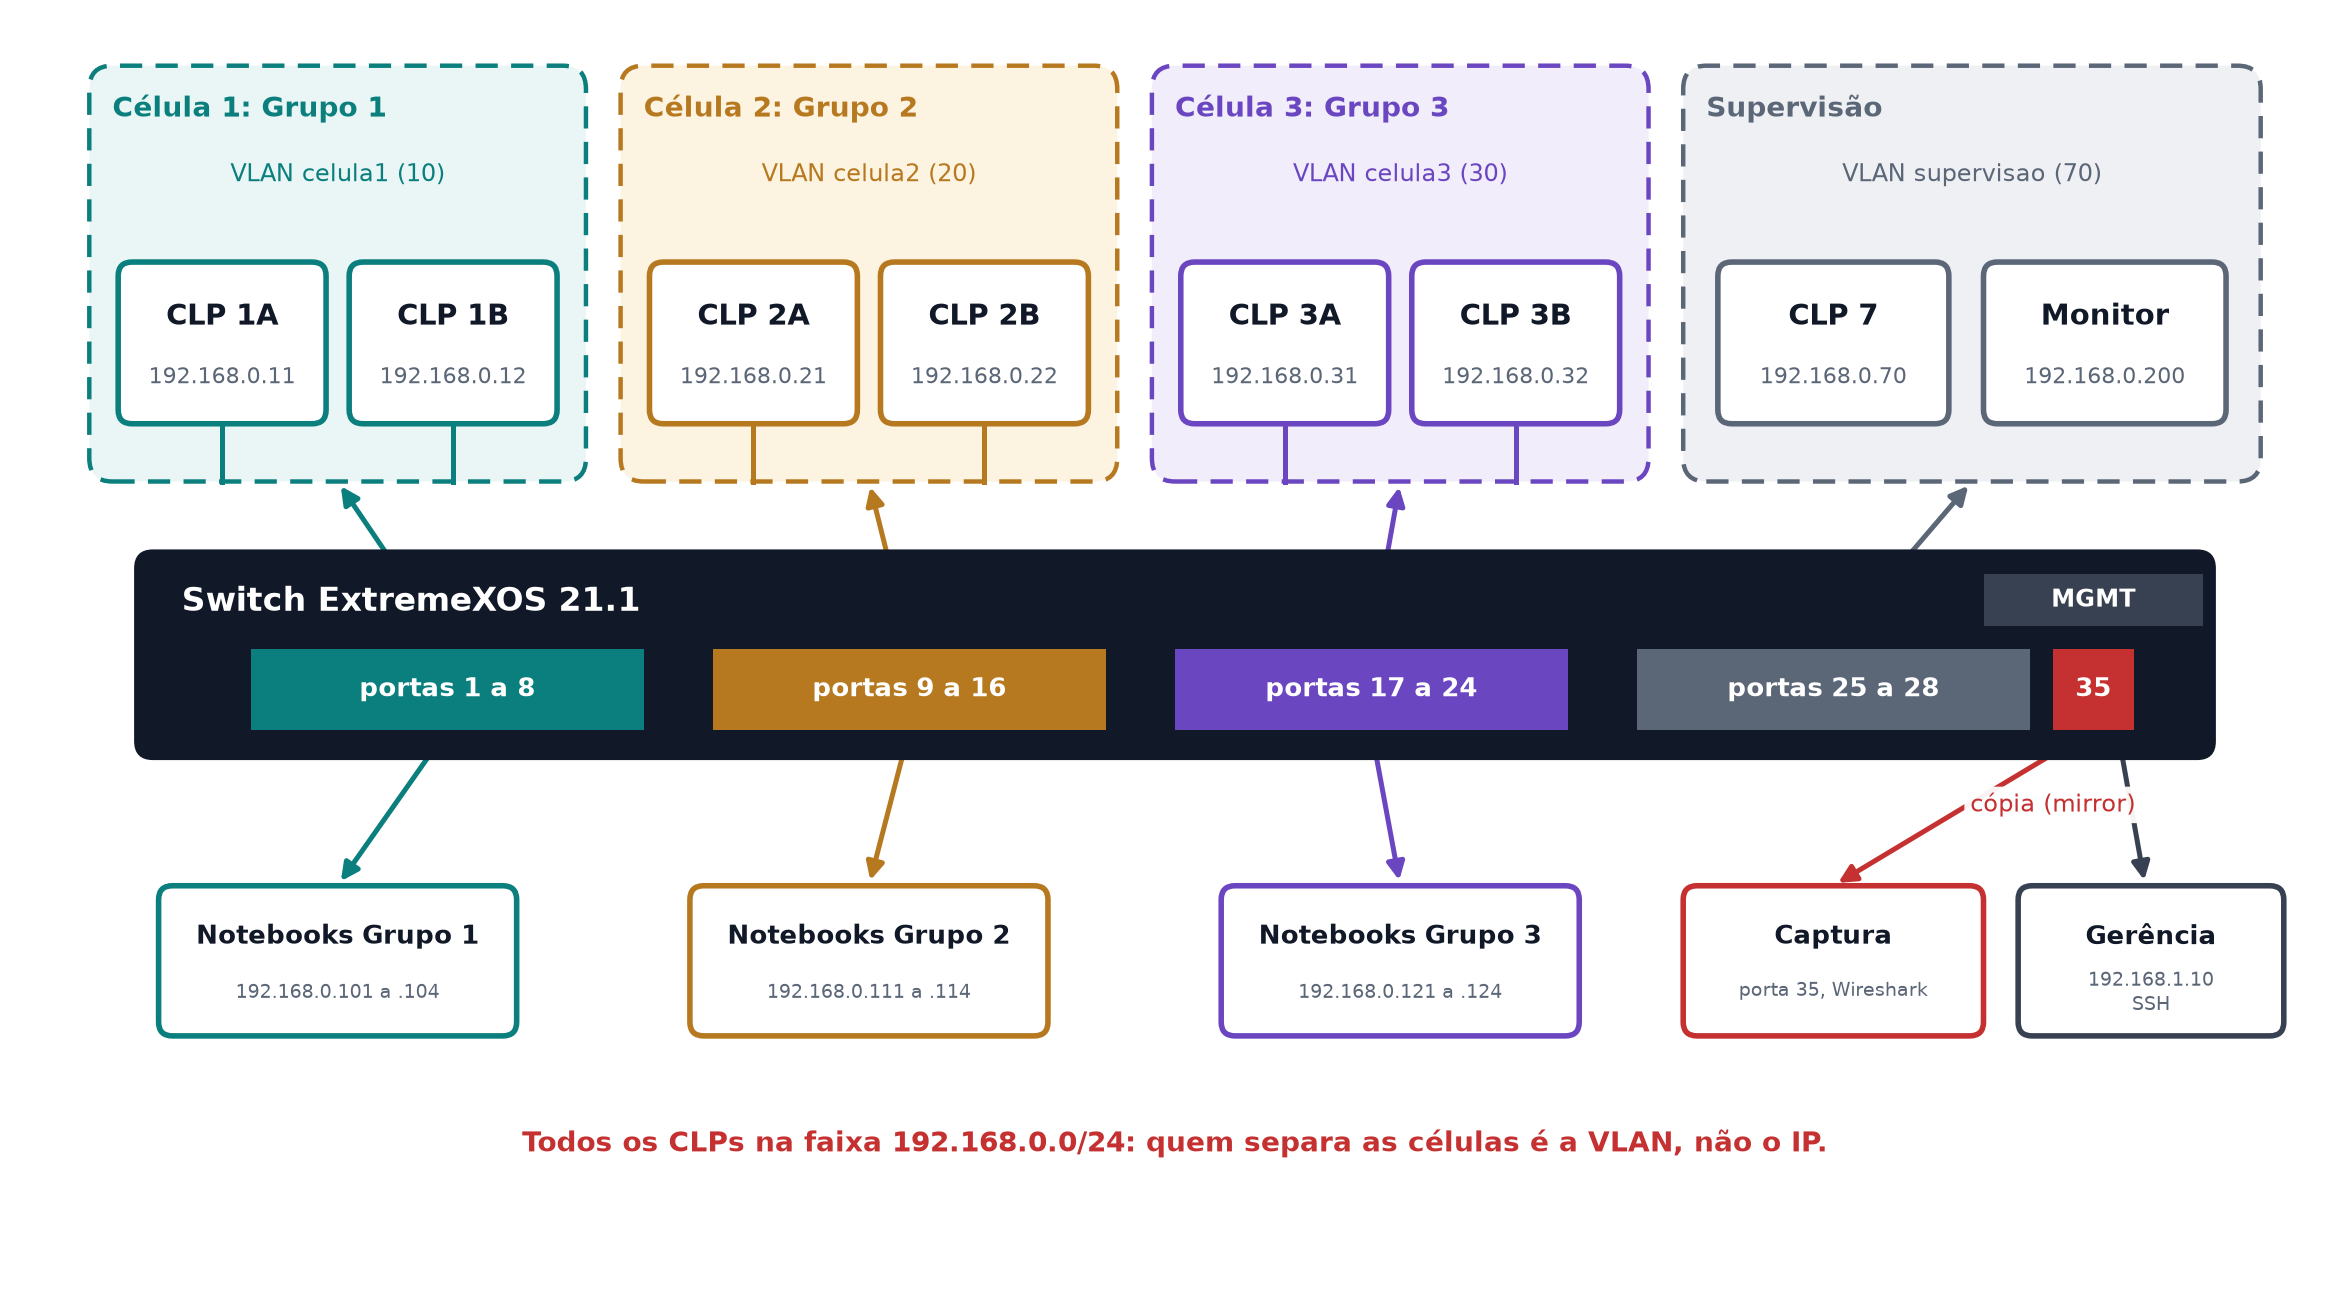
\includegraphics[width=\textwidth]{img/topologia.png}

\vspace{0.3cm}
{\bfseries\color{Navy} Dentro de cada bloco, sempre a mesma ordem}

\small
\begin{tabularx}{\textwidth}{l c c c X}
\rowcolor{Navy}\cab{Posição} & \cab{G1} & \cab{G2} & \cab{G3} & \cab{Uso} \\
1ª & 1 & 9 & 17 & CLP A \\
2ª & 2 & 10 & 18 & CLP B \\
3ª a 6ª & 3--6 & 11--14 & 19--22 & notebooks do grupo \\
7ª e 8ª & 7--8 & 15--16 & 23--24 & livres (desligar na tarefa 4) \\
\bottomrule
\end{tabularx}
\end{minipage}\hfill
\begin{minipage}[t]{0.5\textwidth}
\vspace{0pt}
\small
\begin{tabularx}{\textwidth}{l l l X}
\rowcolor{Navy}\cab{Célula} & \cab{Portas} & \cab{VLAN (tag)} & \cab{IPs} \\
\cel{Ciano} Grupo 1 & 1 a 8 & \texttt{celula1} (10) & CLPs .11 e .12; notebooks .101 a .104 \\
\cel{Ambar} Grupo 2 & 9 a 16 & \texttt{celula2} (20) & CLPs .21 e .22; notebooks .111 a .114 \\
\cel{Roxo} Grupo 3 & 17 a 24 & \texttt{celula3} (30) & CLPs .31 e .32; notebooks .121 a .124 \\
\cel{Cinza} Supervisão & 25 a 28 & \texttt{supervisao} (70) & CLP 7 .70; monitor .200 \\
\cel{Vermelho} Captura & 35 & nenhuma & notebook com Wireshark (saída do mirror \texttt{CAPTURA}) \\
\cel{Navy} Gerência & MGMT & \texttt{mgmt} & switch 192.168.1.10 (só o monitor) \\
\bottomrule
\end{tabularx}

\vspace{0.1cm}
{\footnotesize Todos os IPs começam com \texttt{192.168.0.} e usam máscara \texttt{255.255.255.0}.}

\vspace{0.35cm}
{\bfseries\color{Navy} Rodízio no switch (turnos de cerca de 13 minutos)}

\begin{tabularx}{\textwidth}{l X c c c}
\rowcolor{Navy}\cab{Rodada} & \cab{Tarefa no switch} & \cab{G1} & \cab{G2} & \cab{G3} \\
1 & 1. Mapear e 2. Isolar (VLAN) & 0:45 & 0:58 & 1:11 \\
2 & 3. Monitorar (mirror na porta 35) & 1:25 & 1:38 & 1:51 \\
3 & 4. Endurecer & 2:05 & 2:15 & 2:25 \\
\bottomrule
\end{tabularx}

\vspace{0.1cm}
{\footnotesize Fora do turno: tarefa 0 (PUT/GET no TIA Portal), ficha de comandos, análise da captura.}

\vspace{0.35cm}
{\bfseries\color{Vermelho} Regras do switch}
\begin{itemize}\setlength{\itemsep}{1pt}
\item Cada grupo digita só comandos do \textbf{próprio bloco} de portas.
\item O monitor confere a ficha \textbf{antes} de digitar.
\item \textbf{Nunca} rodar \texttt{save configuration}.
\item No fim da tarefa 3, tirar a sua porta do \texttt{CAPTURA}.
\item Ninguém mexe na porta MGMT nem na VLAN \texttt{mgmt}.
\end{itemize}
\end{minipage}

\end{document}
